\subsection{\texorpdfstring{$y''+(ax^4+bx^3+cx^2+dx+e)y = 
0$}{y''-(ax4+bx3+cx2+dx+e)y = 0}}

Auch ein Polynom $4$-ten Grades stellt kein Problem mehr dar. In die 
Formel \eqref{eq:wellen:allgemeineak} eingesetzt, ergibt sich
\begin{align*}
		a_k &= -\frac{1}{k(k-1)} (aa_{k-2-4} + 
		ba_{k-2-3} + ca_{k-2-2} + da_{k-2-1} +ea_{k-2-0})
		\\
		&= -\frac{1}{k(k-1)} (aa_{k-6} + ba_{k-5} + 
		ca_{k-4} + da_{k-3} +ea_{k-2}), &a_{k<0} &= 0.
\end{align*}

Vergleichen wir die zwei Wellen, die beim Polynom $2$-ten und $4$-ten Grades 
entstehen (Abbildung \ref{fig:wellen:poly4-dgl}), kann man sehen, 
dass im Bereich, wo sich die Profile $p(x)$ "uberlagern, auch die Wellen 
konvergent sind. Da das Polynom $2$-ten Grades zwei Nullstellen besitzt, gibt 
es somit drei Abschnitte zu differenzieren. So haben wir in diesem Fall von 
$-\infty$ bis zur ersten Nullstelle eine Exponentialfunktion, zwischen der 
ersten und zweiten Nullstelle eine Schwingung und danach bis $+\infty$ nochmals 
eine Exponentialfunktion. Beim Polynom $4$-ten Grades sieht dies hingegen etwas 
anders aus, dort gibt es f"unf Abschnitte. Zwischen $-\infty$ und der ersten 
Nullstelle sind die L"osungen des Polynoms positiv, dadurch stellt sich dort 
eine Schwingung ein. Zwischen der ersten und zweiten Nullstelle sind sie 
hingegen negativ, was zu einer Exponentialfunktion f"uhrt. Zwischen der zweiten 
und dritten Nullstelle konvergiert die Welle des Polynom $4$-ten mit derjenigen 
des $2$-ten Grades, was man auch an der Schwingung erkennt. Nach der dritten 
bis zur vierten Nullstelle folgt nochmals eine Exponentialfunktion, die nachher 
bis $+\infty$ in eine Schwingung "uber geht. Dies best"atigt, dass die beim 
parabolischen Profil gefunden Erkenntnisse "uber die Form der L"osungskurve 
allgemein anwendbar sind.

% aus polynom-1-ten-grades.tex hierhin verschoben wegen Buchlayout
\begin{figure}
	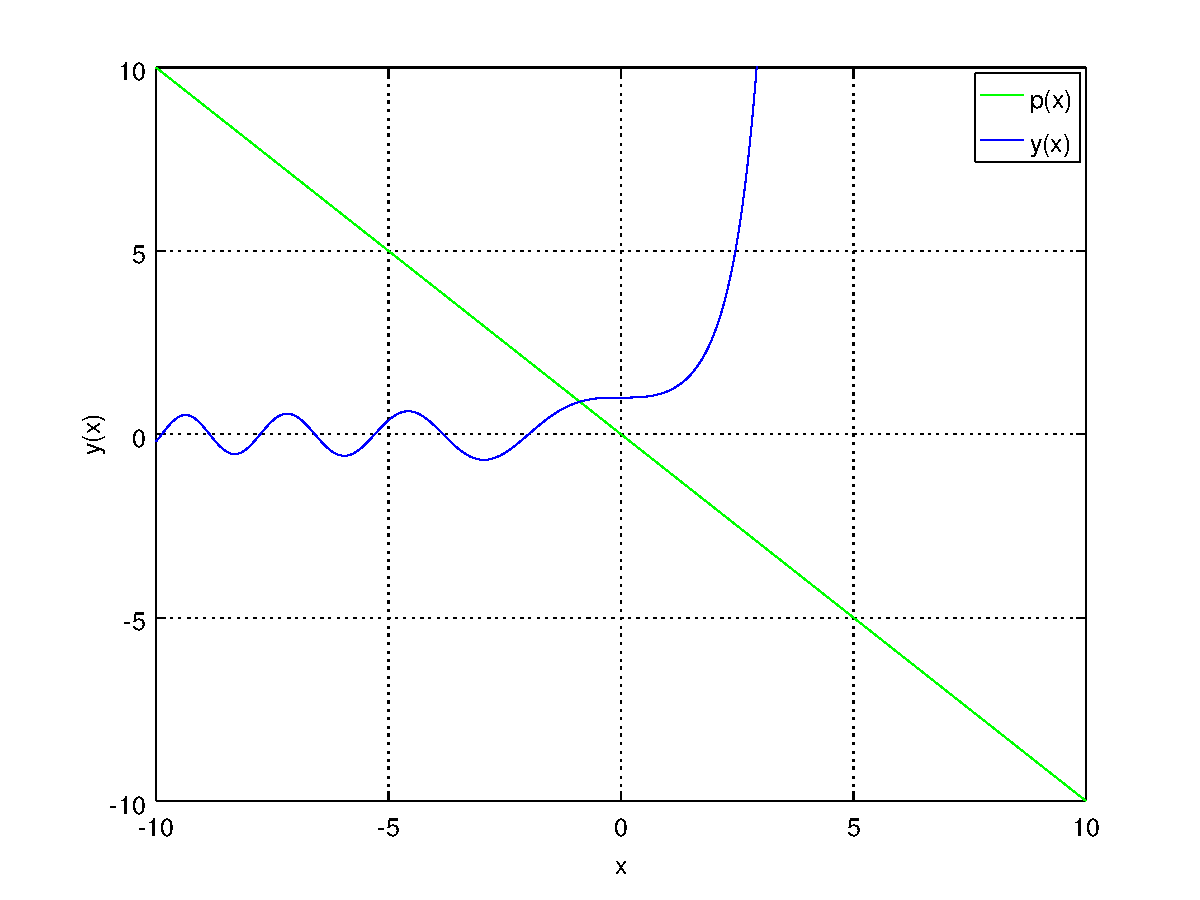
\includegraphics[width=1\hsize]{./wellen/images/allgemein/n1.pdf}
	\caption{L"osung Airy-Differentialgleichung}
	\label{fig:wellen:airy-dgl}
\end{figure}

\begin{figure}
	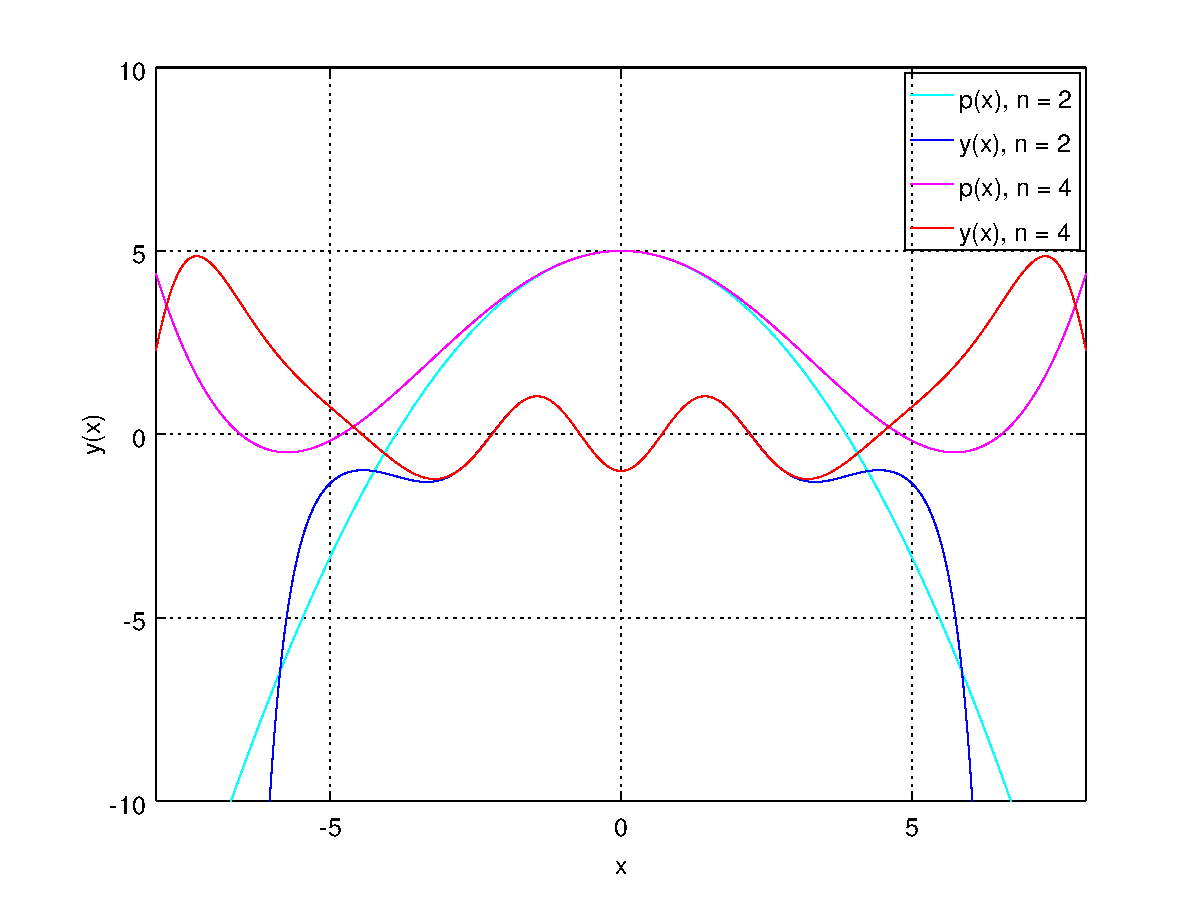
\includegraphics[width=1\hsize]{./wellen/images/allgemein/n4.pdf}
	\caption{Vergleich Polynom 2-ten und 4-ten Grades}
	\label{fig:wellen:poly4-dgl}
\end{figure}
